If current $i_r$ is provided for a time period t then how long the system will keep running with this provided current is defined by the charge to discharge ratio $C_r$ and is given as

\begin{equation}\label{eq:cdr}
 C_r(t) = \frac{i_r(t)}{i_L}
\end{equation}
where $i_r(t) = \frac {5-V_c(t)}{R_c}$ is the current provided for charging at time t and is given by

\begin{equation}\label{eq:ir}
 i_r(t) = \frac {5-V_c(t)}{R_c}
\end{equation}

\begin{figure}[h!]
\centering
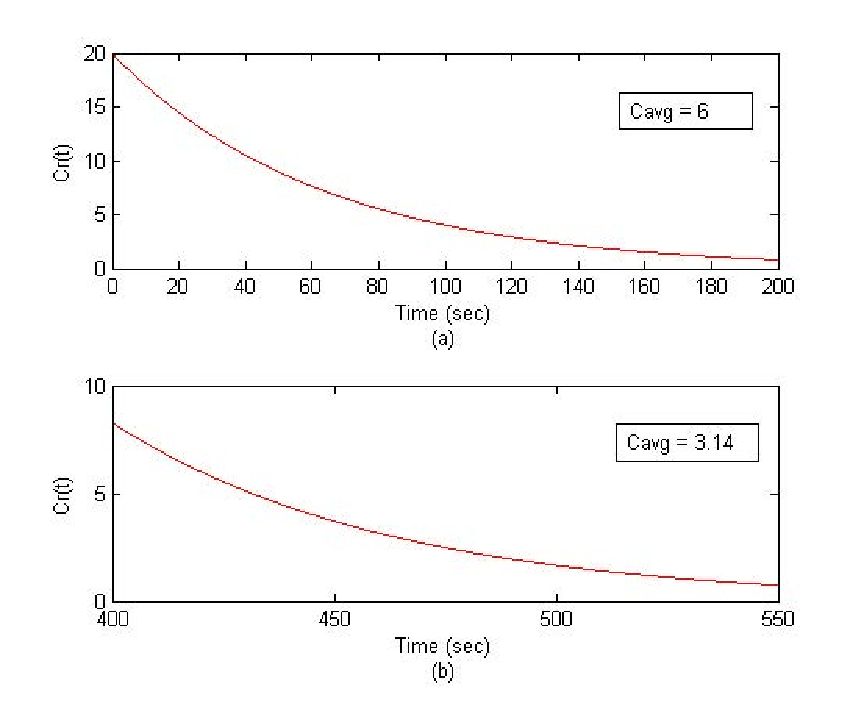
\includegraphics[width=1\textwidth]{ctd2.pdf}
\caption{(a) Charge to discharge ratio for $t_i$ cycle. (b) Charge to discharge ratio for $t_n$ cycle}
\label{fig:crs}
\end{figure}

As $C_r(t)$ is only meaningful during the time when $i_r(t) \neq 0$ which corresponds to time intervals $t_i$ and $t_n$ in the figure \ref{fig:ch_profile}. Hence we can plot $C_r(t)$ for these intervals as shown in figure \ref{fig:crs} (a) and \ref{fig:crs} (b). From figures we can observe that $ C_r(t)$ decreases with time till the value of 2. This is because of the capacitor's charging nature, as $C_s$ starts to charge up,$ V_c(t)$ starts increasing which decreases the value of $ i_r(t)$ [eq:\ref{eq:ir}] and eventually $C_r(t)$. 
To make more meaningful analysis of charge to discharge ratio one can find the average value of $C_r(t)$ using
\begin{equation}\label{eq:cravg}
C_{avg} = \frac{1}{T}\int\limits_t C_r(t) \mathrm{d}t.
\end{equation}
In figures \ref{fig:crs} (a) and (b) for $t_i$ and $t_n$ we can see the value of $ C_{avg}$ to be 6 and 3.14 respectively. The value 3.14 for $t_n$ is of more importance as this value represents the rest of the charging cycles through out the system operation. $i_r(t)$ is responsible for the decrease in $C_r(t)$ which means that the receiving energy is not fully exploited. $C_{avg}$ can be further improved if we can somehow exploit the $i_r(t)$ to its maximum value for all times t. This can be achieved by using a component that can provide constant current regardless of the change at its output voltage. Such components have internal DC to DC convertor and are referred as constant current capacitor/battery chargers. If such a component is added to charge the super capacitor than it is possible to get $i_r(t)$ as constant maximum allowed value for all times t.

\begin{figure}[h!]
\centering
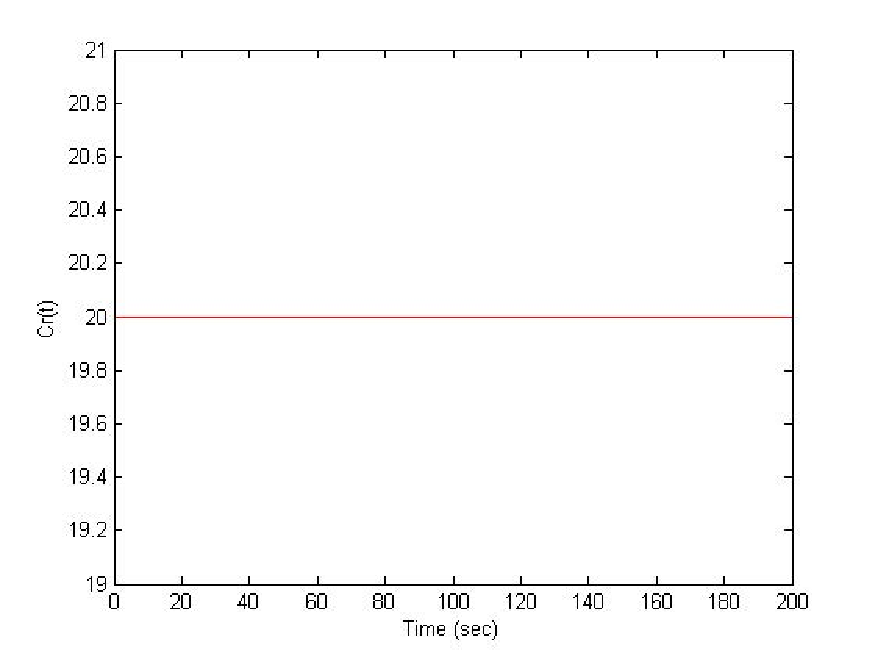
\includegraphics[width=0.8\textwidth]{ctd2c.pdf}
\caption{Charge to discharge ratio with constant charging current $i_r$}
\label{fig:crconst}
\end{figure}

 For constant$ i_r$, $C_r(t)$ profile is shown in figure \ref{fig:crconst}, we can observe that $C_r(t)$ value has been improved to 20 and it stays constant for all values of t.
